%\DeclareMathOperator{\tri}{tri} \DeclareMathOperator{\rect}{rect}
%\DeclareMathOperator{\sgn}{sgn} \DeclareMathOperator{\ramp}{ramp}
%\DeclareMathOperator{\sinc}{sinc}

%\begin{itemize}
%\item Wat betekent het begrip limiet? 
%\item Wanneer is een functie continu in een punt?
%\item Hoe bereken je (eenvoudige) limieten?
%\item Sommige limieten leiden tot onbepaalde vormen (maar kunnen vaak toch
%verder opgelost worden).
%\end{itemize}
\subsection{Het begrip limiet}

Bij het bestuderen van het gedrag van een functie stuiten we soms
op het probleem dat de functie in een bepaald punt niet gedefini\"eerd
is. Dit kan bijvoorbeeld optreden als het voorschrift van de functie
een breuk is waarvan de noemer nul wordt in dat punt. Toch willen
we vaak weten hoe de grafiek van die functie in de buurt van zo'n
punt er uitziet. Ook zijn we ge\"interesseerd in het gedrag van een
functie als het argument zeer groot of zeer sterk negatieve waarden
aanneemt.

Het begrip limiet is dus een belangrijke bouwsteen van de
analyse. De begrippen continu\"iteit, onbepaalde integraal en bepaalde
integraal steunen allen op het limietbegrip. Ook meetkundig is het
limietbegrip van belang: men heeft het nodig bij de definitie van
afgeleiden en asymptoten.


\subsubsection{De verzameling $\bar{\mathbb{R}}$}

Gegeven is de verzameling van de re\"ele getallen $\mathbb{R}$. Stel,
we nemen als deelverzameling het halfopen interval $[5,10[$ van $\mathbb{R}$.
Er bestaat dan bijvoorbeeld een getal uit die verzameling dat kleiner
of gelijk is aan alle elementen uit die deelverzameling. We noteren
dit als $\forall x\in[5,10[$ waarvoor geldt dat $x\ge5$. In dit
geval is het gezochte getal 5. Maar dit is niet altijd zo eenvoudig.




Nemen we de deelverzameling $\{...3,5,7,9\}$ van $\mathbb{R}$.
Welk getal kunnen we vinden dat kleiner is dan alle elementen uit
deze deelverzameling? Het getal 1? Of -1? Of -100? Het antwoord wordt
gevonden door de verzameling uit te breiden met de elementen plus
oneindig ($+\infty$) en min oneindig ($-\infty$).




We zeggen nu dat ``streep R streep'' gelijk is aan: $\overline{\mathbb{R}}=\mathbb{R}\cup\{\text{\textminus\ensuremath{\infty}},+\text{\ensuremath{\infty}}\}$
waarbij $\forall x\in\mathbb{R}$ geldt dat $\text{\textminus\ensuremath{\infty}}<x<+\text{\ensuremath{\infty}}$.




Merk op dat de elementen $\text{\textminus\ensuremath{\infty}}$
en $+\text{\ensuremath{\infty}}$ zelf geen re\"ele getallen zijn. Let
ook op met het symbool $\infty$: afhankelijk van de context kan dit
$"+\infty"$ betekenen, maar ook $"+\infty\:\mathrm{of}\:\text{\textminus\ensuremath{\infty}}"$.
In dit laatste geval schrijven we soms $\pm\infty$.


\subsubsection{Rekenen met $\infty$}

Alhoewel $\text{\textminus\ensuremath{\infty}}$ en $+\text{\ensuremath{\infty}}$
geen re\"ele getallen zijn (maar wel symbolen), kunnen we er toch (mits
enige voorzichtigheid) mee rekenen.



\begin{tabel*}{}
	\centering
	\begin{tabular}{lcc|ll}
		\multicolumn{3}{c|}{vermenigvuldiging} & \multicolumn{2}{c}{optelling}\\
		\hline 
		$a\cdot (+\infty)=+\infty$ & als & $a>0$ & $\pm\infty+a=\pm\infty$ & met $a\in\mathbb{R}$\\
		$a\cdot (+\infty)=-\infty$ & als & $a<0$ &  & \\
		$a\cdot (-\infty)=-\infty$ & als & $a>0$ &  & \\
		$a\cdot (-\infty)=+\infty$ & als & $a<0$ &  & \\
		&  &  &  & \\
		$(+\infty)\cdot (+\infty)=+\infty$ &  &   & $(+\infty)+(+\infty)=+\infty$ & \\
		$(-\infty)\cdot (-\infty)=+\infty$ &  &   & $(-\infty)+(-\infty)=-\infty$ & \\
		$(+\infty)\cdot (-\infty)=-\infty$ &  &   &  & \\
	\end{tabular}
\end{tabel*}




$\frac{1}{\infty}=0$ maar let op: $\frac{1}{0}=\infty$
en dus onbepaald (want $\infty$ is geen re\"eel getal).

Soms maken we nog onderscheid tussen een heel klein positief
of heel klein negatief getal: $\frac{1}{0^{+}}=+\infty$ en $\frac{1}{0^{-}}=-\infty$




De volgende vormen zijn ook onbepaald: $\frac{0}{0}$ en
$\frac{\infty}{\infty}$ , $0\cdot \infty$, $+\infty-\infty$ , $0{}^{0}$
, $\infty{}^{0}$ , $1{}^{\infty}$.

Hoezo, $1{}^{\infty}$ is onbepaald? Dit is toch gewoon
$1\cdot 1\cdot 1\cdot 1\cdot \,\ldots$ en dus gelijk aan $1$!? Het antwoord hierop vind
je op het einde van dit hoofdstukje.

Merk op dat de vormen $\frac{0}{0}$ en $\frac{\infty}{\infty}$
infeite hetzelfde betekenen, immers $\frac{a}{b}$ kan je ook schrijven
als $\frac{\frac{1}{b}}{\frac{1}{a}}$.

\subsection{Intu\"itieve uitleg limieten}
\begin{minipage}{.25\linewidth}
	\raggedright
	
\includegraphics[width=4cm]{2_elem_rekenvaardigheden_B/inputs/QR_Code_LIMIETEN_module2}
\end{minipage}
\begin{minipage}{.7\linewidth}
	Zie filmpje MOOC.
\end{minipage}

\subsection{Limieten en continu\"iteit}

\subsubsection{Het limietbegrip}

Als $x$ nadert tot $a$, dan nadert $f(x)$ tot $b$.

We zeggen wiskundig: de limiet van $f(x)$ voor $x$ gaande
naar $a$ is $b$.

We noteren dit als: $\lim_{x\to a}f(x)=b$

Grafisch:

\gewonefiguur{height=5cm}{2_elem_rekenvaardigheden_B/inputs/limietbegrip}


\begin{voorbeeld}
de functie is continu in $a$ 

$f(x)=x+1$

\gewonefiguur{height=5cm}{2_elem_rekenvaardigheden_B/inputs/limietbegripvb1}


We merken meteen op dat $dom\,f=\mathbb{R}$ (m.a.w. we mogen voor
$x$ elk re\"eel getal kiezen).

Als we $x$ voldoende dicht laten naderen tot bijvoorbeeld $1$, dan
nadert $f(x)$ tot $2$ (zie grafiek).

We noteren dit als: $\lim_{x\to1}f(x)=\lim_{x\to1}(x+1)=2$
en dit is hier ook $=f(1)$.

Omdat $\lim_{x\to1}(x+1)=f(1)$ zeggen we dat deze
functie \textbf{continu} is in het punt $x=1$.

\end{voorbeeld}


\begin{voorbeeld}
de functie is discontinu in $a$

$f(x)=\frac{2x\text{\texttwosuperior}-2x}{x-1}=\frac{2x(x-1)}{x-1}$

De noemer mag niet nul worden. Dus het domein van de functie is: $domf=\mathbb{R}\setminus\{1\}$

\gewonefiguur{height=5cm}{2_elem_rekenvaardigheden_B/inputs/limietbegripvb2}

Als we nu terug $x$ voldoende dicht laten naderen tot $1$, dan nadert
$f(x)$ terug tot $2$ (zie grafiek).

We noteren dit als: $\lim_{x\to1}f(x)= \lim_{x\to1}\frac{2x(x-1)}{x-1}=2$
maar dit is $\neq f(1)$ want 1 behoort niet tot het domein van deze
functie. En toch bestaat de limiet voor $x\rightarrow1$.

Hier is $\lim_{x\to1}\frac{2x(x-1)}{x-1}\neq f(1)$
. De limiet is dus niet gelijk aan de functiewaarde; we zeggen dat
de functie \textbf{niet-continu} of \textbf{discontinu} is in het
punt $x=1$.

\end{voorbeeld}

\subsubsection{Continu versus discontinu}

Een functie $f$ is continu in een \textbf{punt} $x=a$ als: $\lim_{x\to a}f(x)=f(a)$

Het is belangrijk dat je inziet dat voor de limietberekenaar
de functiewaarde niet belangrijk is, immers je gaat naar het punt
$a$ zonder het punt $a$ zelf ooit te bereiken. Dit is het principe
van het limietbegrip. Pas als je gaat kijken naar continu\"iteit moet
je ook rekening houden met (het al dan niet bestaan van) de functiewaarde.


Het is je waarschijnlijk al opgevallen dat we nog niks gezegd
hebben over ``hoe je naar het punt $a$ kan gaan''. Dit kan immers
langs de linkerkant van $a$, of langs de rechterkant van $a$ gebeuren
(we spreken van respectievelijk de linker- en de rechterlimiet).


We noteren: %
\begin{tabular}{l|l}
linkerlimiet & $\lim_{\overset{x\rightarrow a}{<}}f(x)$\\
rechterlimiet & $\lim_{\overset{x\rightarrow a}{>}}f(x)$\\
\end{tabular}

\begin{ftonthoud}
	Twee belangrijke besluiten:
\begin{itemize}
\item als de linkerlimiet en de rechterlimiet beiden bestaan en gelijk zijn
aan elkaar, dan bestaat \textbf{de} limiet $\lim_{x\to a}f(x)$
. De grafiek loopt van beide kanten naar dat punt $(a,f(a))$ toe.
\item als bovendien de limiet ook nog gelijk is aan $f(a)$ dan zit daar
geen discontinu\"iteit (geen gaatje), dus de grafiek bestaat in dat
punt. Dit betekent dat de limiet gelijk is aan de functiewaarde en
dat de functie continu is in het punt $a$.
\end{itemize}
Vereenvoudigd zegt men soms ook dat een functie continu
is als je de grafiek ervan kunt tekenen zonder je potlood van het
papier te halen.
\end{ftonthoud}


Tenslotte zeggen we dat een functie $f$ continu is over
het gesloten interval $[a,b]$ indien:
\begin{itemize}
\item $f$ rechts continu is in $a$ (m.a.w. $\lim_{\overset{x\rightarrow a}{>}}f(x)=f(a)$
)
\item $f$ links continu is in $b$ (m.a.w. $\lim_{\overset{x\rightarrow b}{<}}f(x)=f(b)$
)
\item $\forall x\in]a,b[$ geldt dat $f$ continu is in $x$ (m.a.w. $f(x)$
is continu in elk punt binnen het interval).
\end{itemize}



Je ziet dat een functie $f$ discontinu kan zijn in een
punt $a$ omdat:
\begin{itemize}
\item ze in dat punt niet gedefinieerd is: $f(a)$ bestaat niet
\item ze in dat punt een sprong maakt: $\lim_{\overset{x\rightarrow a}{<}}f(x)$$\neq\lim_{\overset{x\rightarrow a}{>}}f(x)$
\item haar definitie in dat punt niet overeenkomt met de limiet: $\lim_{x\to a}f(x)$$=b\neq f(a)$ 
\item haar waarde onbeperkt toeneemt naarmate men het punt nadert: $\lim_{x\to a}f(x)$$=\pm\infty$ 
\end{itemize}

\subsection{Voorbeelden}

\begin{voorbeeld}
	\ \\
	\gewonefiguur{height=6cm}{2_elem_rekenvaardigheden_B/inputs/Continuvb1}
	
Bestaan de limieten als $x=3$?

\begin{math}
\left. \begin{array}{l}
\lim_{\overset{x\rightarrow3}{<}}g(x) \text{ bestaat niet want dom} \ g=[3,+\infty[\\
 \lim_{\overset{x\rightarrow3}{>}}g(x)=2
\end{array}
\right\}
\Rightarrow \lim_{x\to3}g(x) \text{bestaat niet want } \lim_{\overset{x\rightarrow3}{<}}g(x) \neq \lim_{\overset{x\rightarrow3}{>}}g(x).
\end{math}

Is de functie continu in $x=3$?

\begin{math}
\centering
\left. \begin{array}{l}
g \text{ is niet linkscontinu in }3\\
g \text{ is rechtscontinu in }3
\end{array}
\right\}
\Rightarrow g \text{ is discontinu in }3.
\end{math}

\end{voorbeeld}
\begin{voorbeeld}
	\ \\
\gewonefiguur{width=6cm}{2_elem_rekenvaardigheden_B/inputs/Continuvb2}

Bestaan de limieten in $x=2$?

\begin{math}
\left. \begin{array}{l}
\lim_{\overset{x\rightarrow2}{<}}f(x)=-1 \\
 \lim_{\overset{x\rightarrow2}{>}}f(x)=+1
\end{array}
\right\}
\Rightarrow \lim_{x\to2}f(x) \text{bestaat niet want } \lim_{\overset{x\rightarrow2}{<}}f(x) = \lim_{\overset{x\rightarrow2}{>}}f(x).
\end{math}

Is de functie continu in $x=2$?

\begin{math}
\centering
\left. \begin{array}{l}
g \text{ is niet linkscontinu in }2\\
g \text{ is niet rechtscontinu in }2
\end{array}
\right\}
\Rightarrow f \text{ is discontinu in }2.
\end{math}


\end{voorbeeld}


\begin{voorbeeld}
	\ \\
\gewonefiguur{width=6cm}{2_elem_rekenvaardigheden_B/inputs/Continuvb3}

Bestaan de limieten in $x=1$?

\begin{math}
\left. \begin{array}{l}
\lim_{\overset{x\rightarrow1}{<}}f(x)=5 \\
 \lim_{\overset{x\rightarrow1}{>}}f(x)=5
\end{array}
\right\}
\Rightarrow \lim_{x\to1}f(x) \text{ bestaat en is } 5
\end{math}

Is de functie continu in $x=1$?

\begin{math}
\centering
\left. \begin{array}{l}
f \text{ is niet linkscontinu in }1\\
f \text{ is niet rechtscontinu in }1
\end{array}
\right\}
\Rightarrow f \text{ is discontinu in }1.
\end{math}


\end{voorbeeld}


\begin{voorbeeld}
	\ \\
\gewonefiguur{width=6cm}{2_elem_rekenvaardigheden_B/inputs/Continuvb4}

Bestaan de limieten in $x=2$?

\begin{math}
\left. \begin{array}{l}
\lim_{\overset{x\rightarrow2}{<}}f(x)=+\infty \\
 \lim_{\overset{x\rightarrow2}{>}}f(x)=+\infty
\end{array}
\right\}
\Rightarrow \lim_{x\to2}f(x)=+\infty.
\end{math}

Is de functie continu in $x=2$?

\begin{math}
\centering
\left. \begin{array}{l}
f \text{ is niet linkscontinu in }2\\
f \text{ is niet rechtscontinu in }2
\end{array}
\right\}
\Rightarrow f \text{ is discontinu in }2.
\end{math}

We merken nog op dat $\lim_{x\rightarrow+\infty}f(x)=0$ en $\lim_{x\rightarrow-\infty}f(x)=0$. Hier spreken we over een horizontale asymptoot met vergelijking $y=0$.

\end{voorbeeld}

\begin{voorbeeld}
	\ \\
\gewonefiguur{width=6cm}{2_elem_rekenvaardigheden_B/inputs/Continuvb5}	

Bestaan de limieten in $x=4$?

\begin{math}
\left. \begin{array}{l}
\lim_{\overset{x\rightarrow4}{<}}g(x)=-\infty \\
 \lim_{\overset{x\rightarrow4}{>}}g(x)=+\infty
\end{array}
\right\}
\Rightarrow \lim_{x\to4}g(x) \text{ bestaat niet}.
\end{math}

Is de functie continu in $x=4$?

\begin{math}
\centering
\left. \begin{array}{l}
g \text{ is niet linkscontinu in }4\\
g \text{ is niet rechtscontinu in }4
\end{array}
\right\}
\Rightarrow f \text{ is discontinu in }4.
\end{math}

Er is een verticale asymptoot met vergelijking $x=4$.
Merk verder op dat $\lim_{x\rightarrow+\infty}g(x)=1$ en $\lim_{x\rightarrow-\infty}g(x)=1$.
Er is dus ook een horizontale asymptoot met vergelijking $y=1$.

\end{voorbeeld}

\subsection{Limieten - voorbeeld}

\begin{minipage}{.25\linewidth}
	\raggedright
	
\includegraphics[width=4cm]{2_elem_rekenvaardigheden_B/inputs/QR_Code_LIMIETENVOORBEELD_module2}
\end{minipage}
\begin{minipage}{.7\linewidth}
	Zie filmpje MOOC.
\end{minipage}

\subsection{Limieten van functies (en asymptoten)}


\subsubsection{Limiet bij onbeperkte toename van het argument}

We stellen ons de vraag wat $f(x)$ wordt als we $x$ naar (plus of
min) oneindig laten gaan.

Laten we eerst naar een voorbeeld kijken. 
\begin{voorbeeld}
Stel $f(x)= 1-\frac{1}{x\text{\texttwosuperior}}$

\gewonefiguur{height=5cm}{2_elem_rekenvaardigheden_B/inputs/AsymptootHorizontaal}

We stellen vast dat naarmate $x$ toeneemt, $f(x)$ waarden
aanneemt die onbeperkt dicht bij 1 komen te liggen. Hetzelfde gebeurt
wanneer $x$ negatief is, maar in absolute waarde onbeperkt toeneemt.
We kunnen dit noteren (en berekenen) a.d.h.v. de limietnotatie: $\lim_{x\to+\infty}\left(1-\frac{1}{x\text{\texttwosuperior}}\right)=1$
en $\lim_{x\to-\infty}\left(1-\frac{1}{x\text{\texttwosuperior}}\right)=1$
\end{voorbeeld}

Algemeen:

De afstand tussen de waarden van $f(x)$ en $b$ wordt willekeurig
klein, als het argument $x$ maar voldoende groot wordt (argument
neemt onbeperkt toe of af).


\begin{eqnarray*}
 \lim_{x\to+\infty}f(x)=b & \Leftrightarrow & \forall\varepsilon>0,\:\exists m>0:\:x>m\:\Rightarrow\left|f(x)-b\right|<\varepsilon\\
 \lim_{x\to-\infty}f(x)=b & \Leftrightarrow & \forall\varepsilon>0,\:\exists m>0:\:x<-m\:\Rightarrow\left|f(x)-b\right|<\varepsilon
\end{eqnarray*}

Dit houdt in dat men eerst een willekeurig positief getal $\varepsilon$
kiest en in functie van deze gekozen $\varepsilon$, vastlegt hoe
groot dan $m$ moet zijn. Dit is uitvoerbaar, hoe klein men $\varepsilon$
ook kiest. We kunnen ook zeggen: je kan $f(x)$ oneindig dicht bij
$b$ laten komen, mits je maar een heel grote waarde voor $x$ kiest.

De horizontale rechte met vergelijking $y=b$ noemen we de \textbf{horizontale
asymptoot} van de functie $f(x)$. In ons voorbeeld met de functie
$f(x)= 1-\frac{1}{x\text{\texttwosuperior}}$ is er
\'e\'en horizontale asymptoot met als vergelijking $y=1$. Merk op dat
de functie $f(x)$ deze horizontale rechte (de asymptoot) zowel voor
$x\rightarrow-\infty$ als voor $x\rightarrow+\infty$ langs de onderkant
benadert.

Het is ook mogelijk dat de waarden van $f(x)$ onbeperkt
toenemen, naarmate $x$ toeneemt, denk maar aan de veeltermfunctie
$f(x)=x\text{\texttwosuperior}+1$ of de exponenti\"ele functie $f(x)=3^{x}$.

We stellen vast dat naarmate $x$ toeneemt, ook $f(x)$
onbeperkt toeneemt: $ \lim_{x\to+\infty}3^{x}=+\infty$. 

Merk op dat de limiet van de functie $3^{x}$ voor $x$
gaande naar $\text{\textminus\ensuremath{\infty}}$ gewoon naar $0$
gaat. Dus de rechte met vergelijking $y=0$ is hier dan een horizontale
asymptoot.

\gewonefiguur{height=5cm}{2_elem_rekenvaardigheden_B/inputs/AsymptootOneindig}

Algemeen:

De waarden van $f(x)$ worden groter dan om het even welk (groot)
re\"eel getal, als men $x$ maar voldoende groot neemt (argument neemt
onbeperkt toe of af).

\begin{eqnarray*}
 \lim_{x\to+\infty}f(x)=+\infty & \Leftrightarrow & \forall n>0,\:\exists m>0:\:x>m\:\Rightarrow f(x)>n\\
 \lim_{x\to+\infty}f(x)=-\infty & \Leftrightarrow & \forall n>0,\:\exists m>0:\:x>m\:\Rightarrow f(x)<-n\\
\end{eqnarray*} 

Hierbij legt men eerst vast hoe groot men wil dat $f(x)$ wordt; dit
is het getal $n$. In functie van die gekozen $n$ bepaalt men de
benodigde $m$ .

(gelijkaardige redenering en formuleringen voor $x\rightarrow\text{\textminus\ensuremath{\infty}}$).


\subsubsection{Limiet van een functie wanneer het argument onbeperkt nadert tot
een vaste waarde $a$}

Laten we nu even kijken naar het geval waarbij we $x$ naar een welbepaalde
vaste waarde $a$ laten gaan: ${\displaystyle \lim_{x\to a}}f(x)=b$.
We kunnen alvast zeggen dat $b\in\overline{\mathbb{R}}$.

\begin{voorbeeld}
	Als voorbeeld beschouwen we de functie $f(x)={\displaystyle \frac{5x\text{\texttwosuperior}-5x}{x-1}}={\displaystyle \frac{5x(x-1)}{x-1}}$ 

\gewonefiguur{height=5cm}{2_elem_rekenvaardigheden_B/inputs/Continuvb3}

Wanneer we het argument $x$ laten naderen tot 1, dan stellen
we vast dat $f(x)$ nadert naar 5, en dit zowel langs de linker als
langs de rechterkant van 1.

We schrijven: ${\displaystyle \lim_{\overset{x\rightarrow1}{<}}}{\displaystyle \frac{5x\text{\texttwosuperior}-5x}{x-1}}=5$
en ${\displaystyle \lim_{\overset{x\rightarrow1}{>}}}{\displaystyle \frac{5x\text{\texttwosuperior}-5x}{x-1}}=5$ 

\end{voorbeeld}

Algemeen:

De afstand tussen de waarden $f(x)$ en $b$ wordt willekeurig klein,
als het argument $x$ maar dicht genoeg nabij $a$ komt.

\begin{eqnarray*}
{\displaystyle \lim_{\overset{x\rightarrow a}{<}}}f(x)=b & \Leftrightarrow & \forall\varepsilon>0,\:\exists\delta>0:\:x\in]a-\delta,a[\:\Rightarrow\left|f(x)-b\right|<\varepsilon\\
{\displaystyle \lim_{\overset{x\rightarrow a}{>}}}f(x)=b & \Leftrightarrow & \forall\varepsilon>0,\:\exists\delta>0:\:x\in]a,a+\delta[\:\Rightarrow\left|f(x)-b\right|<\varepsilon\\
\end{eqnarray*}

Hierbij gaat men ervan uit dat men eerst $\varepsilon$ vrij (willekeurig
klein) gekozen heeft en dat men dan $\delta$ bepaalt in functie van
de gekozen $\varepsilon$ .

Het gebruik van deze definitie veronderstelt dat $f(x)$ gedefinieerd
is in een omgeving van $a$ , maar niet noodzakelijk in $a$ zelf
(herinner je dat de limietberekenaar niet ge\"interesseerd is in $f(a)$
)! 

Even terzijde: aangezien in bovenstaand voorbeeld zowel
de linker- als rechterlimiet bestaan en gelijk zijn, bestaat de limiet:
${\displaystyle \lim_{x\to1}}{\displaystyle \frac{5x\text{\texttwosuperior}-5x}{x-1}}=5$.
Maar aangezien deze niet gelijk is aan de functiewaarde $f(1)$, want
$1\notin dom\,f$, kunnen we besluiten dat de functie discontinu is
in het punt $x=1$. Er zit bijgevolg een perforatie (gaatje) in de
grafiek van $f$. Maar we zouden dit 'gat' in het domein kunnen opheffen
door de functiewaarde in $x=1$ 'erbij te defini\"eren': we stellen
de functiewaarde gelijk aan de limiet (zodat de nieuwe, uitgebreide
functie nu wel overal gedefinieerd is, en bovendien overal continu
is). We spreken dan van een ophefbare discontinu\"iteit.

De ``nieuwe'' functie $f(x)$ wordt nu gedefinieerd als:
$f(x):\:\begin{cases}
x\rightarrow\frac{5x\text{\texttwosuperior}-5x}{x-1} & \quad\mathrm{als}\:x\neq1\\
x\rightarrow5 & \quad\mathrm{als}\:x=1
\end{cases}$

Uiteraard is het ook mogelijk dat $f(x)$ onbeperkt toeneemt
als $x$ onbeperkt nadert tot $a$. 

\begin{voorbeeld}
Als voorbeeld bekijken we de functie
$f(x)=\frac{1}{x}$.

\gewonefiguur{height=5cm}{2_elem_rekenvaardigheden_B/inputs/AsymptootVerticaal}

Nadert $x$ langs rechts naar $0$, dit wil zeggen langs
waarden die groter zijn dan nul, dan worden de functiewaarden onbegrensd
groot in positieve zin. $f(x)$ nadert naar plus oneindig als $x$
langs rechts naar $0$ nadert. 

Nadert $x$ langs links naar $0$, dit wil zeggen langs
waarden die kleiner zijn dan nul, dan worden de functiewaarden onbegrensd
groot in negatieve zin. $f(x)$ nadert naar min oneindig als $x$
langs links naar $0$ nadert.


We schrijven: ${\displaystyle \lim_{\overset{x\rightarrow0}{>}}}{\displaystyle \frac{1}{x}}={\displaystyle \frac{1}{0^{+}}}=+\infty$
en ${\displaystyle \lim_{\overset{x\rightarrow0}{<}}}{\displaystyle \frac{1}{x}}={\displaystyle \frac{1}{0^{-}}}=-\infty$

\end{voorbeeld}
Algemeen:

Indien de waarden van $f(x)$ onbeperkt toenemen als $x$ maar dicht
genoeg bij $a$ komt, zegt men:

\begin{eqnarray*}
{\displaystyle \lim_{x\to a}}f(x)=+\infty & \Leftrightarrow & \forall n>0,\:\exists\delta>0:\:0<\left|x-a\right|<\delta\:\Rightarrow f(x)>n\\
{\displaystyle \lim_{x\to a}}f(x)=-\infty & \Leftrightarrow & \forall n>0,\:\exists\delta>0:\:0<\left|x-a\right|<\delta\:\Rightarrow f(x)<-n\\
\end{eqnarray*}

Hierbij gaat men ervan uit dat men eerst $n$ vrij gekozen heeft en
dat men dan $\delta$ bepaalt in functie van de gekozen $n$ .

De verticale rechte met vergelijking $x=a$ noemen we de \textbf{verticale
asymptoot} van de functie $f(x)$. In ons voorbeeld met de functie
$f(x)={\displaystyle \frac{1}{x}}$ is er \'e\'en verticale asymptoot
met als vergelijking $x=0$. Merk op dat de functie $f(x)$ deze verticale
rechte (de asymptoot) voor $x\rightarrow0^{-}$ naar $-\infty$ nadert,
en voor $x\rightarrow0^{+}$ naar $+\infty$ benadert.

\subsection{Epsilon delta definitie voor limieten}
\begin{minipage}{.25\linewidth}
	\raggedright
	
\includegraphics[width=4cm]{2_elem_rekenvaardigheden_B/inputs/QR_Code_EPSILONDELTA_module2}
\end{minipage}
\begin{minipage}{.7\linewidth}
	Zie filmpje MOOC.
\end{minipage}

\subsection{Linkerlimiet en rechterlimiet}

Soms is de waarde van $\lim_{x\to a}f(x)$ afhankelijk
van de manier waarop we naar $a$ naderen. We maken in dat geval een
onderscheid tussen

\begin{table}[h]
\centering
\begin{tabular}{lcl}
	\multirow{2}{*}{de linkerlimiet} & $\lim_{\overset{x\rightarrow a}{<}}f(x)$ & we naderen $a$ langs de te kleine kant van $a$ ($\lyxmathsym{\textquotedblleft}<\lyxmathsym{\textquotedblright}$)\\
	& $\lim_{x\uparrow a}f(x)$ & $x$ stijgt tot aan de waarde van $a$\\
	\multirow{2}{*}{de rechterlimiet} & $\lim_{\overset{x\rightarrow a}{>}}f(x)$ & we naderen $a$ langs de te grote kant van $a$ $(\lyxmathsym{\textquotedblleft}>\lyxmathsym{\textquotedblright}$)\\
	& $\lim_{x\downarrow a}f(x)$ & $x$ daalt tot aan de waarde van $a$\\
\end{tabular}
\end{table}

Wanneer de linker- en rechterlimiet van elkaar verschillen,
zeggen we dat de limiet niet bestaat. 

Enkel als $\lim_{\overset{x\rightarrow a}{<}}f(x)=\lim_{\overset{x\rightarrow a}{>}}f(x)=\lim_{x\to a}f(x)=b\;(\in\mathbb{R})$
zeggen we dat \textbf{de} limiet bestaat.

Zie ook het paragraafje over \emph{continu versus discontinu}.

Redenen om een onderscheid te maken tussen een linker- en
een rechterlimiet kunnen zijn:
\begin{itemize}
\item dat $f(x)$ slechts aan \'e\'en van beide kanten van $a$ bestaat
\item dat naarmate $x$ nadert tot $a$, de waarden die $f(x)$ doorloopt
naar een ander waarde toe leiden naargelang $x$ kleiner of groter
blijft dan $a$ (sprongdiscontinu\"iteit).
\end{itemize}

\begin{voorbeeld}
	
Stel de functie $g(x)=\sqrt{x-4}$

%\begin{figure}[h]
%\centering{}\includegraphics[height=5cm]{\string"2_elem_rekenvaardigheden_B/inputs/Linkerlimiet en rechterlimiet\string".eps} 
%\end{figure}


Deze functie bestaat enkel voor $x\geq4$ (we schrijven $dom\,g=[4,+\infty[$
)

We berekenen de linkerlimiet: $\lim_{\overset{x\rightarrow4}{<}}\sqrt{x-4}$
maar deze bestaat niet.

We berekenen de rechterlimiet: $\lim_{\overset{x\rightarrow4}{>}}\sqrt{x-4}=0$ 

We kunnen besluiten dat de limiet $\lim_{x\to4}\sqrt{x-4}$
niet bestaat (enkel de rechterlimiet bestaat wel).

\end{voorbeeld}

\subsection{Rekenregels}

In de onderstelling dat de limieten bestaan en eindig zijn gelden
de onderstaande rekenregels.

De limieten van $f(x)$ en $g(x)$ bestaan en zijn eindig,
dus: $\lim_{x\to a}f(x)=F$ en $\lim_{x\to a}g(x)=G$.

\begin{ftrekenregel}
	\begin{tabel*}{}
	\centering
	\begin{tabular}{ll}

		1 & $\lim_{x\to a}c=c$ met $c$ een constante ($c\in\mathbb{R}$)\\

		2 & $\lim_{x\to a}x=a$  \\

		3 & $\lim_{x\to a}c\cdot f(x)=c\cdot \lim_{x\to a}f(x)=c\cdot F$  met $c\in\mathbb{R}$\\

		4 & $\lim_{x\to a}\left[f(x)\pm g(x)\right]=\lim_{x\to a}f(x)\pm\lim_{x\to a}g(x)=F\pm G$  \\

		5 & $\lim_{x\to a}\left[f(x)\cdot g(x)\right]=\lim_{x\to a}f(x)\cdot \lim_{x\to a}g(x)=F\cdot G$  \\

		6 & $\lim_{x\to a}\left[\frac{f(x)}{g(x)}\right]=\frac{\lim_{x\to a}f(x)}{\lim_{x\to a}g(x)}=\frac{F}{G}$  mits $\lim_{x\to a}g(x)\neq0$\\

		7 & $\lim_{x\to a}\left[f\left(g(x)\right)\right]=f\left(\lim_{x\to a}g(x)\right)$  mits $f$ continu is in het punt $\lim_{x\to a}g(x)=b$ \\


	\end{tabular}
\end{tabel*}
\end{ftrekenregel}

Eigenschap 7 in woorden: het omwisselen van het nemen van
de limiet en het nemen van de functiewaarde door de functie $f$ is
enkel toegestaan als $f$ een continue functie is in het betreffende
punt. We zeggen ook wel eens \textquoteleft de limiet passeert de functie $f$\textquoteright.

\textbf{Tip1}: de rekenregels voor $\infty$ zijn vrij eenvoudig
te onthouden en te gebruiken als $(+)\infty$ gelezen wordt als \textquoteleft een
heel groot (positief) getal\textquoteright, $-\infty$ als 'een heel groot negatief
getal', $0^{+}$ als \textquoteleft een heel klein positief getal\textquoteright en tenslotte $0^{-}$
als \textquoteleft een heel klein negatief getal\textquoteright.

\textbf{Tip2}: lees bijvoorbeeld de rekenregels 4, 5 en 6 ook eens
op een andere manier: ``de limiet van een som, is de som van de limieten''
...

\begin{voorbeeld}
\begin{eqnarray*}
\lim_{x\to+\infty}\frac{x}{4}&=&\frac{1}{4} \lim_{x\to+\infty}x=\frac{1}{4}\cdot (+\infty)=+\infty\\
\lim_{x\to3}\left[(x-2)(x+1)\right]&=& \lim_{x\to3}(x-2)\cdot  \lim_{x\to3}(x+1)=1\cdot 4=4\\
\lim_{x\to3}(x\text{\texttwosuperior}-x-2)&=& \lim_{x\to3}x\text{\texttwosuperior}- \lim_{x\to3}x-2\cdot  \lim_{x\to3}1=9-3-2=4\\
\lim_{\overset{x\rightarrow0}{>}}\left(2x-\frac{1}{x}\right)&=& \lim_{\overset{x\rightarrow0}{>}}2x- \lim_{\overset{x\rightarrow0}{>}}\frac{1}{x}=2\cdot 0-\left(+\infty\right)=-\infty\\
\lim_{x\to a}\left[\cos\left(g(x)\right)\right]&=&\cos\left( \lim_{x\to a}g(x)\right)\\
\lim_{x\to a}\left[e^{f(x)}\right]&=&e^{\lim_{x\to a}f(x)}
\end{eqnarray*}
\end{voorbeeld}

\subsection{Berekenen van limieten}

\subsubsection{Veeltermfuncties}

Een veeltermfunctie van n\textsuperscript{de} graad:

\begin{equation*}
f(x)=a_{n}x^{n}+a_{n-1}x^{n-1}+\ldots+a_{2}x^{2}+a_{1}x+a_{0}\text{ met }
a_{n}\in\mathbb{R}_{0}\text{ en }a_{n-1},\ldots,a_{0}\in\mathbb{R}
\end{equation*}

Elke veeltermfunctie is continu over $\mathbb{R}$ (want
het domein is immers $\mathbb{R}$).

De limiet voor $x$ gaande naar $a\in\overline{\mathbb{R}}$
van een veeltermfunctie is gelijk aan de functiewaarde (m.a.w. vervang
overal $x$ door $a$):

\begin{equation*}
\lim_{x\to a}\left(a_{n}x^{n}+a_{n-1}x^{n-1}+\ldots+a_{2}x^{2}+a_{1}x+a_{0}\right)=f(a)
\end{equation*}

Een speciaal geval is de limiet voor $x$ gaande naar oneindig.
In dit geval is het infeite enkel de hoogste graad term die van belang
is. Kijk maar:

\begin{eqnarray*}
\lim_{x\to+\infty}\left(a_{n}x^{n}+a_{n-1}x^{n-1}+\ldots+a_{1}x+a_{0}\right)&=& \lim_{x\to+\infty}a_{n}x^{n}\left(1+\frac{a_{n-1}x^{n-1}}{a_{n}x^{n}}+\ldots+\frac{a_{1}x}{a_{n}x^{n}}+\frac{a_{0}}{a_{n}x^{n}}\right) \\
&=& \lim_{x\to+\infty}a_{n}x^{n}(1+0+\ldots+0)\\
&=& \lim_{x\to+\infty}a_{n}x^{n}
\end{eqnarray*}


\begin{voorbeeld}
\begin{eqnarray*}
\lim_{x\to+\infty}\left(-x\text{\textthreesuperior}+6x+14\right)&=& \lim_{x\to+\infty}x\text{\textthreesuperior}\left(-1+\frac{6x}{x\text{\textthreesuperior}}+\frac{14}{x\text{\textthreesuperior}}\right)\\
&=& \lim_{x\to+\infty}x\text{\textthreesuperior}\left(-1\right)\\
&=&-\infty\\
& & \\
\lim_{x\to-\infty}\left(3x\text{\texttwosuperior}-4x+2\right)&=& \lim_{x\to-\infty}3x\text{\texttwosuperior}\left(1-\frac{4x}{3x\text{\texttwosuperior}}+\frac{2}{3x\text{\texttwosuperior}}\right)\\
&=&\lim_{x\to-\infty}3x\text{\texttwosuperior}\\
&=&+\infty
\end{eqnarray*}
\end{voorbeeld}

\subsubsection{Goniometrische en cyclometrische functies}

Laat ons meteen opmerken dat bij de berekeningen van deze limieten
het argument van de goniometrische of cyclometrische functie moet
uitgedrukt zijn in radialen. 

Enkele van deze limieten geven in eerste instantie aanleiding
tot de onbepaalde vorm $\frac{0}{0}$, maar toch kan men de limiet
vinden. We bekijken als voorbeeld de limiet van $ \lim_{x\to0}\frac{\sin x}{x}$.
Maken we een tabel met $x$-waarden die steeds dichter naar $0$ naderen,
dan zien we dat de verhouding $\frac{\sin x}{x}$ naar 1 gaat.

\begin{tabel*}{}
	\centering
	\begin{tabular}{l|l}
		$x$ & $\frac{\sin x}{x}$\\
		\hline 
		1 & 0,84147098480\\
		0,1 & 0,99833416646\\
		0,01 & 0,99998333341\\
		0,001 & 0,99999983333\\
		0,0001 & 0,99999999999\\
	\end{tabular}
\end{tabel*}


Aangezien $\lim_{\overset{x\rightarrow0}{<}}\frac{\sin x}{x}=\lim_{\overset{x\rightarrow0}{>}}\frac{\sin x}{x}=1$
kunnen we concluderen dat $\lim_{x\rightarrow0}\frac{\sin x}{x}=1$
(hetzelfde geldt trouwens ook voor $\lim_{x\rightarrow0}\frac{x}{\sin x}=1$
).


De limiet $\lim_{x\rightarrow\infty}\frac{\sin x}{x}=0$
kunnen we dan weer wiskundig bewijzen a.d.h.v. de zogenaamde insluitstelling.
Het komt er hierbij op neer dat je probeert een functie in te sluiten
tussen twee andere functies die beide een gelijke limiet $L$ hebben.
De limiet van de ingesloten functie is dan ook gelijk aan $L$.

We weten dat de sinus-functie altijd een waarde oplevert
tussen -1 en +1: $-1\leq\sin x\leq+1$.

Dit blijft gelden als we de vergelijking delen door een
positieve $x$ waarde: $\frac{-1}{x}\leq\frac{\sin x}{x}\leq\frac{+1}{x}$.

We weten ook dat: $\lim_{x\to\infty}\left(\frac{-1}{x}\right)=0$
en $\lim_{x\to\infty}\left(\frac{1}{x}\right)=0$.

Passen we nu de insluitstelling toe dan concluderen we dat
$\lim_{x\rightarrow\infty}\frac{\sin x}{x}=0$.


De limiet $\lim_{x\rightarrow0}\frac{\sin x}{x}=1$
noemen we een \textquoteleft standaardlimiet\textquoteright, en we kunnen hiermee een andere standaardlimiet
afleiden:

\begin{eqnarray*}
\lim_{x\rightarrow0}\frac{\tan x}{x}&=&\lim_{x\rightarrow0}\frac{\frac{\sin x}{\cos x}}{x}\\
&=&\lim_{x\rightarrow0}\frac{\sin x}{x\cdot \cos x}\\
&=&\lim_{x\rightarrow0}\frac{\sin x}{x}\cdot \lim_{x\rightarrow0}\frac{1}{\cos x}\\
&=&1\cdot \frac{1}{1}=1
\end{eqnarray*}


\begin{voorbeeld}

\begin{equation*}
\lim_{x\rightarrow0}\frac{\tan2x}{\sin3x}=\lim_{x\rightarrow0}\frac{\tan2x}{\sin3x}\cdot \frac{2x}{2x}\cdot \frac{3x}{3x}=\lim_{x\rightarrow0}\frac{\tan2x}{2x}\cdot \frac{2}{3}\cdot \frac{3x}{\sin3x}=\frac{2}{3}
\end{equation*}

\end{voorbeeld}



Nog enkele veel voorkomende limieten van goniometrische
en cyclometrische functies (tip: kijk ook eens naar hun grafiek of
de goniometrische cirkel)

\begin{table}[ht]
	\centering
	\begin{tabular}{c|c|c}
		$\lim_{\overset{x\rightarrow\frac{\pi}{2}}{<}}\tan x=+\infty$ & $\lim_{x\rightarrow+\infty}\arctan x=\frac{\pi}{2}$ & $\lim_{\overset{x\rightarrow1}{<}}\arcsin x=\frac{\pi}{2}$\\
		$\lim_{\overset{x\rightarrow-\frac{\pi}{2}}{>}}\tan x=-\infty$ & $\lim_{x\rightarrow-\infty}\arctan x=-\frac{\pi}{2}$ & $\lim_{\overset{x\rightarrow-1}{>}}\arcsin x=-\frac{\pi}{2}$\\
		$\lim_{\overset{x\rightarrow0}{<}}\cot x=-\infty$ & $\lim_{x\rightarrow+\infty}\mathrm{arccot}x=0$ & $\lim_{\overset{x\rightarrow1}{<}}\arccos x=0$\\s
		$\lim_{\overset{x\rightarrow0}{>}}\cot x=+\infty$  & $\lim_{x\rightarrow-\infty}\mathrm{arccot}x=\pi$ & $\lim_{\overset{x\rightarrow-1}{>}}\arccos x=\pi$\\
	\end{tabular}
\end{table}

\begin{minipage}{.5\linewidth}
	\gewonefiguur{width=\linewidth}{2_elem_rekenvaardigheden_B/inputs/Arctangent_Arccotangent_svg}
\end{minipage}
\begin{minipage}{.5\linewidth}
	\gewonefiguur{width=.7\linewidth}{2_elem_rekenvaardigheden_B/inputs/Arcsine_Arccosine_svg}
\end{minipage}

\subsubsection{Exponenti\"ele en logaritmische functies}

Deze limieten laten zich gemakkelijk afleiden uit de grafieken:

Exponenti\"ele functies

\begin{tabel*}{}
	\centering
	\begin{tabular}{c|c}
		$a>1$ &  $0<a<1$\\
%		\gewonefiguur{width=7cm}{expagroter1} & 		\gewonefiguur{width=7cm}{expakleiner1} \\
		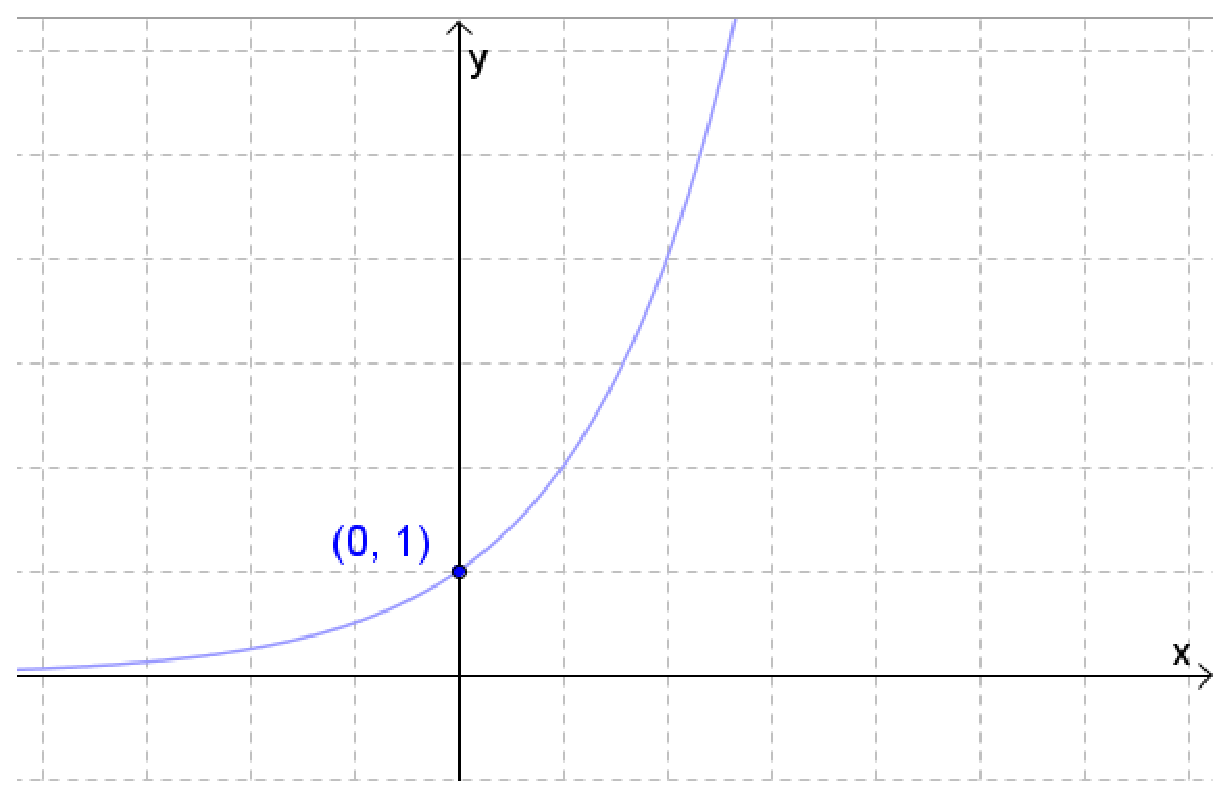
\includegraphics[width=7cm]{2_elem_rekenvaardigheden_B/inputs/expagroter1.eps} & 
		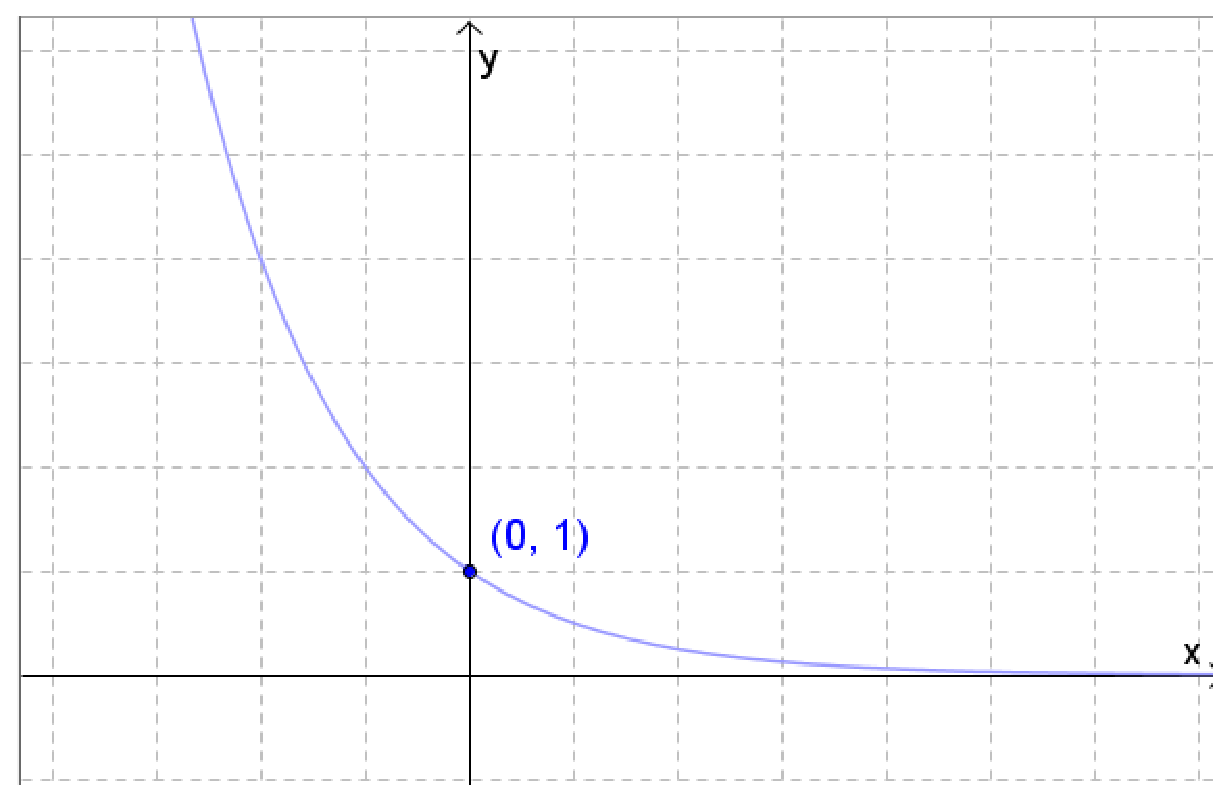
\includegraphics[width=7cm]{2_elem_rekenvaardigheden_B/inputs/expakleiner1.eps}\\
		$\lim_{x\to+\infty}a^{x}=+\infty$ &  $\lim_{x\to+\infty}a^{x}=0$\\
		$\lim_{x\to0}a^{x}=1$ &  $\lim_{x\to0}a^{x}=1$\\
		$\lim_{x\to-\infty}a^{x}=0$ &  $\lim_{x\to-\infty}a^{x}=+\infty$\\
	\end{tabular}
\end{tabel*}

Logaritmische functies

\begin{tabel*}{}
	\centering
	\begin{tabular}{c|c}
		$a>1$ & $0<a<1$\\
		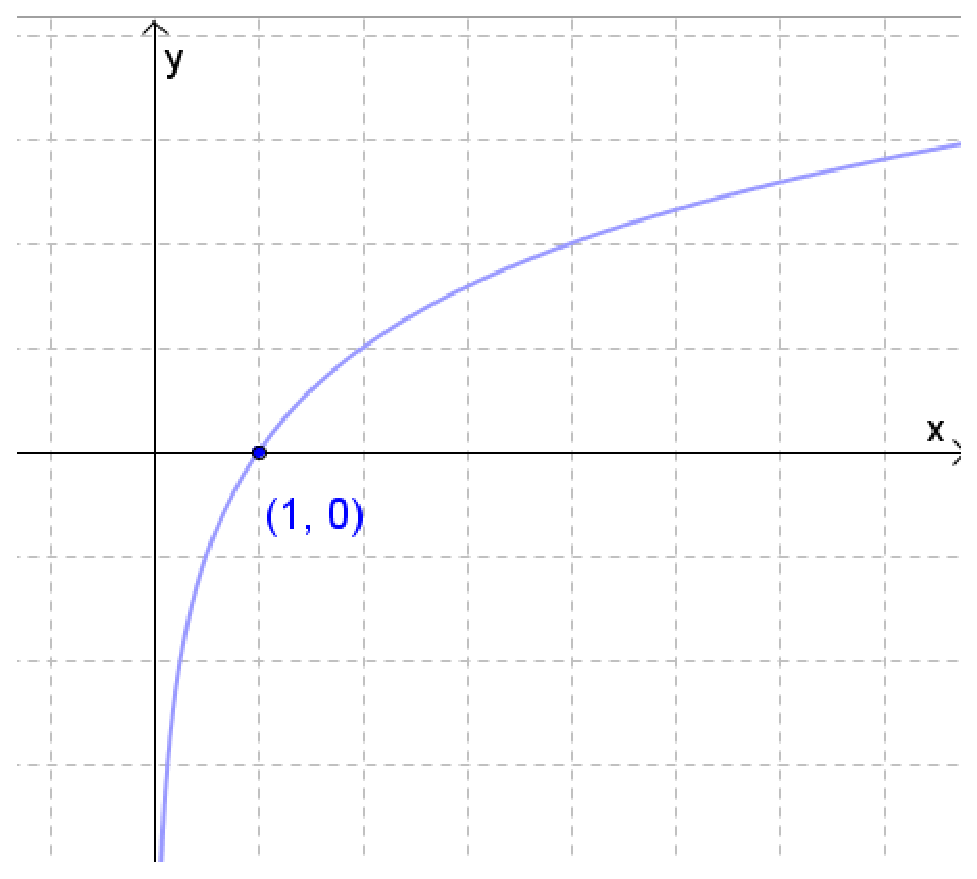
\includegraphics[width=7cm]{2_elem_rekenvaardigheden_B/inputs/logagroter1.eps} & 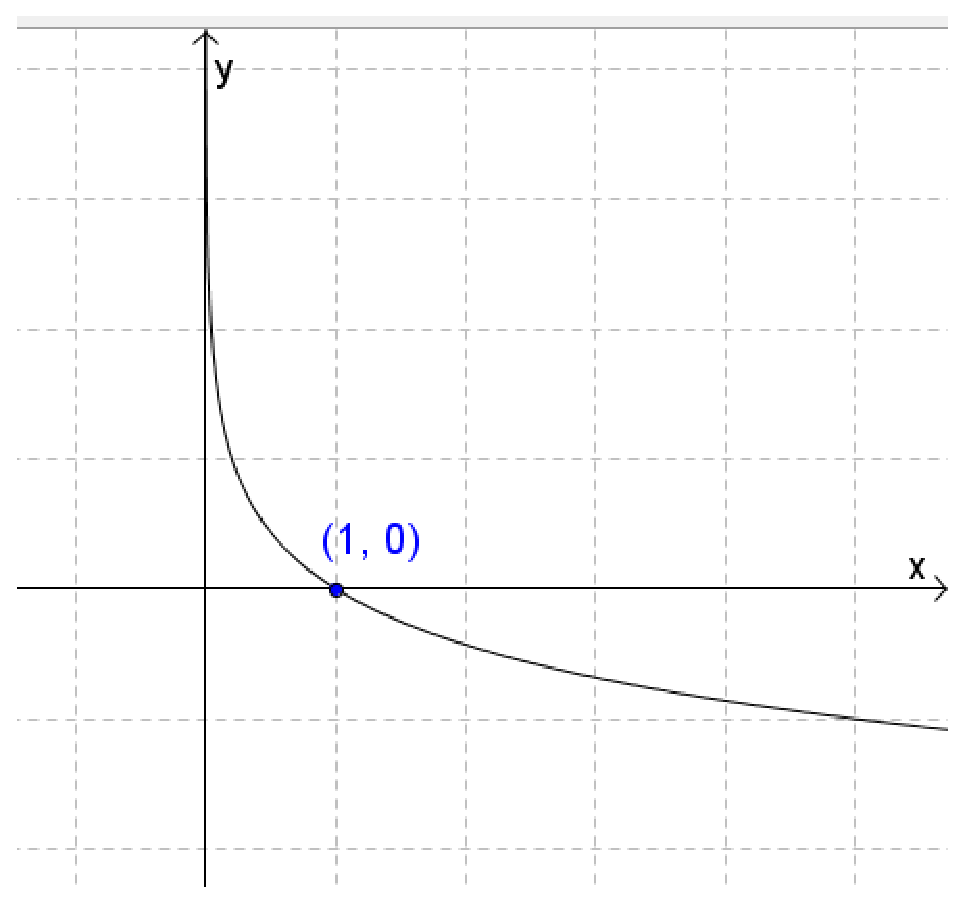
\includegraphics[width=7cm]{2_elem_rekenvaardigheden_B/inputs/logakleiner1}\\
		${\displaystyle \lim_{x\to+\infty}}\log_{a}x=+\infty$ & ${\displaystyle \lim_{x\to+\infty}}\log_{a}x=-\infty$\\
		${\displaystyle \lim_{x\to1}}\log_{a}x=0$ & ${\displaystyle \lim_{x\to1}}\log_{a}x=0$\\
		${\displaystyle \lim_{\overset{x\rightarrow0}{>}}}\log_{a}x=-\infty$ & ${\displaystyle \lim_{\overset{x\rightarrow0}{>}}}\log_{a}x=+\infty$\\
	\end{tabular}
\end{tabel*}

\subsubsection{Enkele bijzondere limieten}
\label{sec:bijzlim}
Een bijzondere limiet is:

\begin{equation*}
\lim_{x\to0}\left(1+x\right)^{\frac{1}{x}}=e=2,718281828...
\text{ en ook } \lim_{x\to\pm\infty}\left(1+\frac{1}{x}\right)^{x}=e
\end{equation*}

Hier zie je ook al waarom we gezegd hebben dat $1^{\infty}$
niet zomaar gelijk is aan 1.

Deze bijzondere limiet kan worden uitgebreid naar:

\begin{equation*}
\lim_{x\to0}\left(1+px\right)^{\frac{q}{x}}=e^{pq}\text{ met }p,q\in\mathbb{R}_{0}\text{ en ook } \lim_{x\to\pm\infty}\left(1+\frac{p}{x}\right)^{qx}=e^{pq}
\end{equation*}

\subsection{Schijnbare onbepaaldheden}

\subsubsection{Onbepaalde vormen}

Om de limiet ${\displaystyle \lim_{x\to a}}f(x)$ te berekenen moeten
we dikwijls onbepaaldheden wegwerken. Daartoe gaan we opzoek naar
functies die gelijkwaardig zijn met de oorspronkelijke functie, maar
bij berekening van de limiet geen aanleiding meer geven tot een onbepaaldheid.

Soms kan een onbepaalde vorm omgezet worden naar een andere
(eveneens onbepaalde) vorm: ${\displaystyle 0.\infty=\frac{1}{\frac{1}{0}}.\infty=\frac{1}{\infty}.\infty=\frac{\infty}{\infty}}$.

Hetzelfde geldt voor de factor oneindig: ${\displaystyle 0.\infty=0.\frac{1}{\frac{1}{\infty}}=0.\frac{1}{0}=\frac{0}{0}}$.

We merken hier meteen op dat een andere aanpak om de onbepaaldheden
$\frac{0}{0}$ en $\frac{\infty}{\infty}$ te evalueren de regel van
de l'H\^opital is.

Limieten van functies van het type $f(x)^{g(x)}$ kunnen
aanleiding geven tot de onbepaalde vormen $0{}^{0}$ , $\infty{}^{0}$
en $1{}^{\infty}$. In deze gevallen kan het herschrijven van de functie
een oplossing bieden: ${\displaystyle f(x)^{g(x)}=e^{\ln f(x)^{g(x)}}=e^{g(x).\ln f(x)}}$.
De functie $g(x).\ln f(x)$ leidt dan vaak tot iets van het type $0.\infty$.


\subsubsection{De onbepaalde vorm $\frac{\infty}{\infty}$}

\begin{itemize}
\item{Rationale functies}

We spreken van rationale functies, als $f(x)$ een quoti\"ent
van is van twee veeltermen. Rationale functies zijn niet gedefinieerd
in de eventuele nulpunten van de noemer; ze hebben daar geen functiewaarde.
Het domein van een rationale functie is $\mathbb{R}$, met uitzondering
van de verzameling nulpunten van de noemer. Elke rationale functie
is continu over zijn domein.

Bij een rationale breuk die een onbepaalde vorm oplevert
van het type $\frac{\infty}{\infty}$ omdat het argument naar $\infty$
streeft, hanteert men volgende regel: 

beschouw in teller en noemer enkel de hoogstegraadstermen en bepaal
de limiet van hun verhouding.



\begin{equation*}
{\displaystyle \lim_{x\to\infty}}\left(\frac{a_{n}x^{n}+a_{n-1}x^{n-1}+\ldots+a_{1}x+a_{0}}{b_{p}x^{p}+b_{p-1}x^{p-1}+\ldots+b_{1}x+b_{0}}\right)={\displaystyle \lim_{x\to\infty}}{\displaystyle \frac{a_{n}x^{n}}{b_{p}x^{p}}} = 
\left\{
\begin{array}{ll}
\pm\infty &\text{ als } n>p \\
\frac{a_n}{b_p} &\text{ als } n=p \\
0 &\text{ als } n<p
\end{array}
\right.
\end{equation*}

%\begin{tabular}{|l|l|c|c|}
%	\hline 
%	${\displaystyle \lim_{x\to\infty}}\left(\frac{a_{n}x^{n}+a_{n-1}x^{n-1}+\ldots+a_{1}x+a_{0}}{b_{p}x^{p}+b_{p-1}x^{p-1}+\ldots+b_{1}x+b_{0}}\right)={\displaystyle \lim_{x\to\infty}}{\displaystyle \frac{a_{n}x^{n}}{b_{p}x^{p}}}$ & $=\infty${*} & als & $n>p$\\
%	\hline 
%	& $={\displaystyle \frac{a_{n}}{b_{p}}}$ & als & $n=p$\\
%	\hline 
%	& $=0$ & als & $n<p$\\
%	\hline 
%\end{tabular}

Merk op dat het teken van $\pm\infty$ moet nog nader bepaald worden.

\begin{voorbeeld}
	
\begin{equation*}
{\displaystyle \lim_{x\to-\infty}}{\displaystyle \frac{2x\text{\textthreesuperior}-11}{x\text{\texttwosuperior}+x-10}}={\displaystyle \lim_{x\to-\infty}}{\displaystyle \frac{2x\text{\textthreesuperior}}{x\text{\texttwosuperior}}}={\displaystyle \lim_{x\to-\infty}}2x=-\infty
\end{equation*}

\begin{equation*}
{\displaystyle \lim_{x\to+\infty}}{\displaystyle \frac{6-x\text{\texttwosuperior}}{2x\text{\texttwosuperior}+5}}={\displaystyle \lim_{x\to+\infty}}{\displaystyle \frac{-x\text{\texttwosuperior}}{2x\text{\texttwosuperior}}}={\displaystyle \lim_{x\to+\infty}}{\displaystyle \frac{-1}{2}}={\displaystyle -\frac{1}{2}}
\end{equation*}

\end{voorbeeld}




\item{Irrationale functies}

Een irrationale functie is een functie waarin wortelvormen van rationale
functies voorkomen. Elke irrationale functie is continu over haar
domein. De uitdrukking onder het wortelteken van een even machtswortel
moet wel positief zijn!

Bij een irrationale breuk die een onbepaalde vorm oplevert
van het type $\frac{\infty}{\infty}$ omdat het argument naar $\infty$
streeft, hanteert men volgende regel:

zet in teller en noemer de hoogst mogelijke macht van $x$ voorop
en werk verder uit.

Hierbij maken we gebruik van het feit dat: 
\begin{equation*}
\sqrt{x^{2}}=\left|x\right|=\begin{cases}
x & \mathrm{als}\:x>0\\
-x & \mathrm{als}\:x<0
\end{cases}
\end{equation*}


\begin{voorbeeld}
	\begin{equation*}
	{\displaystyle {\displaystyle \lim_{x\to\infty}}\frac{\sqrt{x\text{\texttwosuperior}+1}-2x}{\sqrt[3]{x\text{\textthreesuperior}+1}}={\displaystyle \lim_{x\to\infty}}\frac{\left|x\right|\sqrt{1+\frac{1}{x\text{\texttwosuperior}}}-2x}{\sqrt[3]{x\text{\textthreesuperior}}\left(\sqrt[3]{1+\frac{1}{x\text{\textthreesuperior}}}\right)}}
	\end{equation*}

Nu moeten we een onderscheid maken tussen de limiet gaande naar $+\infty$
en $-\infty$:

\begin{equation*}
	{\displaystyle {\displaystyle \lim_{x\to+\infty}}\frac{x\sqrt{1+\frac{1}{x\text{\texttwosuperior}}}-2x}{x\left(\sqrt[3]{1+\frac{1}{x\text{\textthreesuperior}}}\right)}={\displaystyle \lim_{x\to+\infty}}\frac{\sqrt{1+\frac{1}{x\text{\texttwosuperior}}}-2}{\sqrt[3]{1+\frac{1}{x\text{\textthreesuperior}}}}=\frac{1-2}{1}=-1}
\end{equation*}
	en
	\begin{equation*}
{\displaystyle {\displaystyle \lim_{x\to-\infty}}\frac{(-x)\sqrt{1+\frac{1}{x\text{\texttwosuperior}}}-2x}{x\left(\sqrt[3]{1+\frac{1}{x\text{\textthreesuperior}}}\right)}={\displaystyle \lim_{x\to-\infty}}\frac{-\sqrt{1+\frac{1}{x\text{\texttwosuperior}}}-2}{\sqrt[3]{1+\frac{1}{x\text{\textthreesuperior}}}}=\frac{-1-2}{1}=-3}
\end{equation*}

\end{voorbeeld}



\begin{voorbeeld}
	\begin{equation*}
{\displaystyle {\displaystyle \lim_{x\to\infty}}\frac{3x+2}{4x-\sqrt{x\text{\texttwosuperior}+3}}={\displaystyle \lim_{x\to\infty}}\frac{x\left(3+\frac{2}{x}\right)}{4x-\left|x\right|\sqrt{1+\frac{3}{x\text{\texttwosuperior}}}}}
\end{equation*}

We maken terug onderscheid tussen de limiet gaande naar $+\infty$
en $-\infty$:
\begin{equation*}
{\displaystyle \lim_{x\to+\infty}}{\displaystyle \frac{x\left(3+\frac{2}{x}\right)}{4x-x\sqrt{1+\frac{3}{x\text{\texttwosuperior}}}}={\displaystyle \lim_{x\to+\infty}}{\displaystyle \frac{3+\frac{2}{x}}{4-\sqrt{1+\frac{3}{x\text{\texttwosuperior}}}}=\frac{3}{4-1}=1}}
\end{equation*} en

\begin{equation*}
{\displaystyle \lim_{x\to-\infty}}{\displaystyle \frac{x\left(3+\frac{2}{x}\right)}{4x-(-x)\sqrt{1+\frac{3}{x\text{\texttwosuperior}}}}={\displaystyle \lim_{x\to-\infty}}{\displaystyle \frac{3+\frac{2}{x}}{4+\sqrt{1+\frac{3}{x\text{\texttwosuperior}}}}=\frac{3}{4+1}=\frac{3}{5}}}
\end{equation*}

\end{voorbeeld}
\end{itemize}

\subsubsection{De onbepaalde vorm $\frac{0}{0}$}

\begin{itemize}
\item{Rationale functies}

Bij de limiet van een rationale functie in het punt $a$, waarbij
$a$ het nulpunt is van zowel de teller als noemer, zal zowel teller
als noemer als limiet nul hebben. We zullen in teller en noemer de
factoren $(x-a)$ af zonderen en daarna deze factor $(x-a)$ wegdelen.
Daarom gaan we eerst op zoek naar gemeenschappelijke factoren in teller
en noemer; eventueel kan de regel van Horner helpen bij het ontbinden
van de veelterm in factoren.


\begin{voorbeeld}
\begin{equation*}
{\displaystyle {\displaystyle \lim_{x\to2}}\frac{x\text{\texttwosuperior}-4}{x\text{\texttwosuperior}-7x+10}=\frac{0}{0}}
\end{equation*}

Teller en noemer ontbinden in factoren:

teller: $x\text{\texttwosuperior}-4=(x-2)(x+2)$

noemer (via Horner): %
\begin{tabular}{cc|ccc}
	&  & $1$ & $-7$ & $10$\\
	& $2$ & $\downarrow$ & $2$ & $-10$\\
	\cline{2-5} 
	&  & $1$ & \multicolumn{1}{c||}{$-5$} & $0$\\
\end{tabular}

dus \begin{equation*}
x\text{\texttwosuperior}-7x+10=(x-2)(x-5)
\end{equation*}

zodat \begin{equation*}
{\displaystyle {\displaystyle \lim_{x\to2}}\frac{x\text{\texttwosuperior}-4}{x\text{\texttwosuperior}-7x+10}={\displaystyle \lim_{x\to2}}\frac{(x-2)(x+2)}{(x-2)(x-5)}={\displaystyle \lim_{x\to2}}\frac{(x+2)}{(x-5)}=\frac{2+2}{2-5}=-\frac{4}{3}}
\end{equation*}
\end{voorbeeld}


\begin{voorbeeld}
	\begin{equation*}
{\displaystyle {\displaystyle \lim_{x\to3}}\frac{x\text{\texttwosuperior}-9}{x\text{\texttwosuperior}+x-12}=\frac{0}{0}}
\end{equation*}

Teller en noemer ontbinden in factoren:

teller: $x\text{\texttwosuperior}-9=(x-3)(x+3)$

noemer (via Horner): %
\begin{tabular}{cc|ccc}
	&  & $1$ & $1$ & $-12$\\
	& $3$ & $\downarrow$ & $3$ & $12$\\
	\cline{2-5} 
	&  & $1$ & \multicolumn{1}{c||}{$4$} & $0$\\
\end{tabular}

dus \begin{equation*}
x\text{\texttwosuperior}+x-12=(x-3)(x+4)
\end{equation*}

zodat \begin{equation}
{\displaystyle {\displaystyle \lim_{x\to3}}\frac{x\text{\texttwosuperior}-4}{x\text{\texttwosuperior}-7x+10}={\displaystyle \lim_{x\to3}}\frac{(x-3)(x+3)}{(x-3)(x+4)}={\displaystyle \lim_{x\to3}}\frac{(x+3)}{(x+4)}=\frac{3+3}{3+4}=\frac{6}{7}}
\end{equation}
\end{voorbeeld}


\item{Irrationale functies}

Wanneer het nul worden van teller of noemer veroorzaakt wordt door
het aftrekken of het optellen van wortelvormen, zal men teller en
noemer met eenzelfde factor vermenigvuldigen. Deze factor wordt zo
gekozen dat zijn product met de irrationale uitdrukking die nul werd,
nu rationaal zal worden. Men noemt deze factor \emph{een toegevoegde}.


\begin{voorbeeld}
	\begin{equation*}
{\displaystyle {\displaystyle \lim_{x\to3}}\frac{\sqrt{x+1}-2}{x-3}=\frac{0}{0}}
\end{equation*}

De teller gaan we rationaal maken door de teller (en de noemer) te
vermenigvuldigen met $\left(\sqrt{x+1}+2\right)$:

\begin{equation*}
\begin{array}{cl}
{\displaystyle {\displaystyle \lim_{x\to3}}\frac{\sqrt{x+1}-2}{x-3}} & {\displaystyle ={\displaystyle \lim_{x\to3}}\frac{\sqrt{x+1}-2}{x-3}.\frac{\sqrt{x+1}+2}{\sqrt{x+1}+2}}\\
& {\displaystyle ={\displaystyle \lim_{x\to3}}\frac{\left(x+1-4\right)}{\left(x-3\right).\left(\sqrt{x+1}+2\right)}}\\
& {\displaystyle ={\displaystyle \lim_{x\to3}}\frac{x-3}{\left(x-3\right).\left(\sqrt{x+1}+2\right)}}\\
& {\displaystyle ={\displaystyle \lim_{x\to3}}\frac{1}{\sqrt{x+1}+2}}\\
& =\frac{1}{4}
\end{array}
\end{equation*}
\end{voorbeeld}

\begin{voorbeeld}
	\begin{equation*}
{\displaystyle {\displaystyle \lim_{x\to2}}\frac{x-2}{\sqrt{x+7}-3}=\frac{0}{0}}
\end{equation*}

De noemer gaan we rationaal maken door de noemer (en de teller) te
vermenigvuldigen met $\left(\sqrt{x+7}+3\right)$:

\begin{equation*}
\begin{array}{cl}
{\displaystyle {\displaystyle \lim_{x\to2}}\frac{x-2}{\sqrt{x+7}-3}} & {\displaystyle ={\displaystyle \lim_{x\to2}}\frac{x-2}{\sqrt{x+7}-3}.\frac{\sqrt{x+7}+3}{\sqrt{x+7}+3}}\\
& {\displaystyle ={\displaystyle \lim_{x\to2}}\frac{\left(x-2\right).\left(\sqrt{x+7}+3\right)}{\left(x+7-9\right)}}\\
& {\displaystyle ={\displaystyle \lim_{x\to2}}\frac{\left(x-2\right).\left(\sqrt{x+7}+3\right)}{x-2}}\\
& {\displaystyle ={\displaystyle \lim_{x\to2}}\left(\sqrt{x+7}+3\right)}\\
& =6
\end{array}
\end{equation*}
\end{voorbeeld}

\end{itemize}


\subsubsection{De onbepaalde vorm $\infty-\infty$}

Bij irrationale functies vermenigvuldig je met en deel je door de
toegevoegde irrationale vorm (en hoop je op die manier de onbepaaldheid
weg te werken).

\begin{voorbeeld}
\begin{equation*}
{\displaystyle {\displaystyle \lim_{x\to\pm\infty}}\left(\sqrt{x\text{\texttwosuperior}+1}-\sqrt{x\text{\texttwosuperior}-x+3}\right)=\infty-\infty}
\end{equation*}
(zowel voor $x\rightarrow+\infty$ als voor $x\rightarrow-\infty$)

We vermenigvuldigen met het toegevoegde: \begin{equation*}
\left(\sqrt{x\text{\texttwosuperior}+1}+\sqrt{x\text{\texttwosuperior}-x+3}\right)
\end{equation*}

\begin{equation*}
 \begin{array}{cl}
 				{\displaystyle {\displaystyle \lim_{x\to\pm\infty}}\left(\sqrt{x\text{\texttwosuperior}+1}-\sqrt{x\text{\texttwosuperior}-x+3}\right).\frac{\left(\sqrt{x\text{\texttwosuperior}+1}+\sqrt{x\text{\texttwosuperior}-x+3}\right)}{\left(\sqrt{x\text{\texttwosuperior}+1}+\sqrt{x\text{\texttwosuperior}-x+3}\right)}} & {\displaystyle ={\displaystyle \lim_{x\to\pm\infty}}\frac{x\text{\texttwosuperior}+1-(x\text{\texttwosuperior}-x+3)}{\left(\sqrt{x\text{\texttwosuperior}+1}+\sqrt{x\text{\texttwosuperior}-x+3}\right)}}\\
 				 & {\displaystyle ={\displaystyle \lim_{x\to\pm\infty}}\frac{x-2}{\left(\sqrt{x\text{\texttwosuperior}+1}+\sqrt{x\text{\texttwosuperior}-x+3}\right)}}
\end{array}
\end{equation*}

Nu moeten we een onderscheid maken tussen de limiet gaande naar $+\infty$
en $-\infty$:

\begin{equation*}
{\displaystyle {\displaystyle \lim_{x\to+\infty}}\frac{x-2}{\left(\sqrt{x\text{\texttwosuperior}+1}+\sqrt{x\text{\texttwosuperior}-x+3}\right)}={\displaystyle \lim_{x\to+\infty}}\frac{x\left(1-\frac{2}{x}\right)}{x\left(\sqrt{1+\frac{1}{x\text{\texttwosuperior}}}+\sqrt{1-\frac{x}{x\text{\texttwosuperior}}+\frac{3}{x\text{\texttwosuperior}}}\right)}=\frac{1}{2}}
\end{equation*} en

\begin{equation*}
{\displaystyle {\displaystyle \lim_{x\to-\infty}}\frac{x-2}{\left(\sqrt{x\text{\texttwosuperior}+1}+\sqrt{x\text{\texttwosuperior}-x+3}\right)}={\displaystyle \lim_{x\to-\infty}}\frac{x\left(1-\frac{2}{x}\right)}{(-x)\left(\sqrt{1+\frac{1}{x\text{\texttwosuperior}}}+\sqrt{1-\frac{x}{x\text{\texttwosuperior}}+\frac{3}{x\text{\texttwosuperior}}}\right)}=-\frac{1}{2}}
\end{equation*}

\end{voorbeeld}

\begin{voorbeeld}
\begin{equation*}
\lim_{x\to\pm\infty}\left(\sqrt{2x\text{\texttwosuperior}+5}-x\right)
\end{equation*}

Hier maken we meteen onderscheid tussen de limiet gaande naar $+\infty$
en $-\infty$ (omdat de limiet voor $x\rightarrow-\infty$ eigenlijk
geen probleem oplevert) :
\begin{equation*}
\lim_{x\to-\infty}\left(\sqrt{2x\text{\texttwosuperior}+5}-x\right)=+\infty-(-\infty)=+\infty
\end{equation*}

\begin{eqnarray*}
\lim_{x\to+\infty}\left(\sqrt{2x\text{\texttwosuperior}+5}-x\right) & =&+\infty-(+\infty)\:\mathrm{dus...}\\
 &=& {\displaystyle {\displaystyle \lim_{x\to+\infty}}\left(\sqrt{2x\text{\texttwosuperior}+5}-x\right)\cdot \frac{\sqrt{2x\text{\texttwosuperior}+5}+x}{\sqrt{2x\text{\texttwosuperior}+5}+x}}\\
 &=& {\displaystyle {\displaystyle \lim_{x\to+\infty}}\frac{2x\text{\texttwosuperior}+5-x\text{\texttwosuperior}}{\sqrt{2x\text{\texttwosuperior}+5}+x}}\\
 &=& {\displaystyle {\displaystyle \lim_{x\to+\infty}}\frac{x\text{\texttwosuperior}+5}{\sqrt{2x\text{\texttwosuperior}+5}+x}}\\
 &=& {\displaystyle {\displaystyle \lim_{x\to+\infty}}\frac{x\text{\texttwosuperior}(1+\frac{5}{x\text{\texttwosuperior}})}{(+x)\sqrt{2+\frac{5}{x\text{\texttwosuperior}}}+x}}\\
 &=& {\displaystyle {\displaystyle \lim_{x\to+\infty}}\frac{x(1+\frac{5}{x\text{\texttwosuperior}})}{\sqrt{2+\frac{5}{x\text{\texttwosuperior}}}+1}}\\
 &=&+\infty
\end{eqnarray*}

\end{voorbeeld}

\subsubsection{De onbepaalde vorm $1^{\infty}$}

We hebben ons reeds eerder verbaasd over het feit dat $1{}^{\infty}$
niet zomaar hetzelfde is als $1\cdot 1\cdot 1\cdot 1\cdot \,\ldots$ en dus niet zomaar
gelijk hoeft te zijn aan $1$!?

De reden is eigenlijk heel eenvoudig: we zitten hier in
het hoofdstukje ``Limieten'', met andere woorden zowel $1$ als
$\infty$ kunnen het resultaat zijn van het nemen van een limiet:
\begin{equation*}
{\displaystyle \lim_{x\to a}f(x)^{g(x)}=\ldots=1^{\infty}}.
\end{equation*}

Laten we, om deze module af te sluiten, kijken naar een
numeriek voorbeeldje. In paragraaf \ref{sec:bijzlim}
hebben we gezien dat: 
\begin{equation*}
{\displaystyle \lim_{x\to0}}\left(1+x\right)^{\frac{1}{x}}=e=2,718281828...
\text{ en ook }{\displaystyle \lim_{x\to\pm\infty}}\left(1+\frac{1}{x}\right)^{x}=e
\end{equation*}

\begin{table}[ht]
\centering
\begin{tabular}{lrcl|lrcl}
	$x$ & \multicolumn{3}{c|}{$\left(1+x\right)^{\frac{1}{x}}$}  & $x$ & \multicolumn{3}{c}{$\left(1+\frac{1}{x}\right)^{x}$}\\
	\hline 
	1 & $2^{1}$ & = & 2,0  & 1 & $2^{1}$ & = & 2,0\\
	0,1 & $1,1^{10}$ & = & 2,59374246  & 10 & $1,1^{10}$ & = & 2,59374246\\
	0,01 & $1,01^{100}$ & = & 2,70481382  & 100 & $1,01^{100}$ & = & 2,70481382\\
	0,0001 & $1,0001^{10000}$ & = & 2,71814592  & 10000 & $1,0001^{10000}$ & = & 2,71814592\\
\end{tabular}
\end{table}



We zien dat, afhankelijk van de vorm die we bekijken, als
$x$ heel dicht bij $0$ of bij oneindig nadert, de vorm schijnbaar
naar $1^{\infty}$ gaat, maar de echte waarde gaat echter naar het
``magische getal $e$''.

